\documentclass[11pt]{article}
\usepackage{amsmath,amssymb,amsthm}
\usepackage{fancyhdr}

% margins
\usepackage[vmargin=1in,hmargin=1.5in]{geometry}

% Drawing for Kmaps
\usepackage{tikz}
\usetikzlibrary{calc}
\usetikzlibrary{positioning}
\usetikzlibrary{matrix}
\pgfdeclarelayer{background}
\pgfsetlayers{background,main}

% Circuit diagrams
\usepackage{circuitikz}

% Config
%%%%%%%%%%%%%%%%%%%%%%%%%%%%%%%%%%%
\newcommand{\lab}{4}
\newcommand{\name}{Connor Taffe}
\newcommand{\tno}{3742} % last 4 digits of T number.
%%%%%%%%%%%%%%%%%%%%%%%%%%%%%%%%%%%

\title{
	$L_{\lab}$ \\
	{\large Laboratory \rom{\lab}} \\
	{\normalsize Prof. Dr. P. Tang, CS 3482: Comp. Org. I}
}
\author{
	\name, T no. \tno
}

\pagestyle{fancy}
\rhead{Lab {\rom{\lab}}}
\lhead{{\name}. T no. \tno}

\usepackage{hw}

\begin{document}
\maketitle

\section{Details of Lab 4}

\begin{question}
	{\bf C}. Change the gate-delay of the {\sc and} gate to 0, 3, 5. Observe the output
	changes with respect to the changes of input $x$.

	The output mimics the input $x$ with an offset along the time axis associated with the time
	of the gate delay. E.g. a 3ns gate delay results in a 3ns shift between the input $x$ and the
	output.
\end{question}

\begin{question}
	Draw the circuit to implement the Boolean function as follows
	\begin{equation}
		\label{eq:booleanexpression}
		f(a,b,c,d) = (a' + b)'c + d(b' + ac)
	\end{equation}
	according to the expression directly.
	Connect $b$, $c$ and $d$ to binary switches and make them to be 0, 1 and 0, respectively.
	Connect $a$ to a clock.

	\begin{subquestion}
		According to your simulation, how much time does it take for the change of $a$ to be
		reflected in the output $f$?

		Five nanoseconds.
	\end{subquestion}

	\begin{subquestion}
		Change the gate delays of all the gates along the path from $a$ to $f$ to 0, 2 and 4.
		Verify that the total delays from $a$ to $f$ you observed are correct.

		For a 0ns delay, $a$ and $f$ corresponded exactly. For a 2ns delay, $a$ and $f$ differed by a 10ns delay.
		For a 5ns delay, $a$ and $f$ differed by a 45ns delay.
	\end{subquestion}


\end{question}

\begin{question}

	Here follows the logical truth table (figure \ref{fig:ttable}), Karnaugh map (figure \ref{fig:kmap}), and direct circuit
	implementation (figure \ref{fig:cdiagram}) of said K. map of equation \ref{eq:booleanexpression}.

	% Logical Truth Table
	\begin{figure}[h]
		\begin{center}
			\begin{tabular} {c c c c | c c c c c c c}
				$a$ & $b$ & $c$ & $d$ & $a'+b$ & $(a'+b)'c$ & $ac$ & $b'+ac$ & $d(b'+ac)$ & $(a'+b)'c+d(b'+ac)$ \\
				\hline
				1 & 1 & 1 & 1 & 1 & 0 & 1 & 1 & 1 & 1 \\
				1 & 1 & 1 & 0 & 1 & 0 & 1 & 1 & 0 & 0 \\
				1 & 1 & 0 & 1 & 1 & 0 & 0 & 0 & 0 & 0 \\
				1 & 1 & 0 & 0 & 1 & 0 & 0 & 0 & 0 & 0 \\
				1 & 0 & 1 & 1 & 0 & 1 & 1 & 1 & 1 & 1 \\
				1 & 0 & 1 & 0 & 0 & 1 & 1 & 1 & 0 & 1 \\
				1 & 0 & 0 & 1 & 0 & 0 & 0 & 1 & 1 & 1 \\
				1 & 0 & 0 & 0 & 0 & 0 & 0 & 1 & 0 & 0 \\
				0 & 1 & 1 & 1 & 1 & 0 & 0 & 0 & 0 & 0 \\
				0 & 1 & 1 & 0 & 1 & 0 & 0 & 0 & 0 & 0 \\
				0 & 1 & 0 & 1 & 1 & 0 & 0 & 0 & 0 & 0 \\
				0 & 1 & 0 & 0 & 1 & 0 & 0 & 0 & 0 & 0 \\
				0 & 0 & 1 & 1 & 1 & 0 & 0 & 1 & 1 & 1 \\
				0 & 0 & 1 & 0 & 1 & 0 & 0 & 1 & 0 & 0 \\
				0 & 0 & 0 & 1 & 1 & 0 & 0 & 1 & 1 & 1 \\
				0 & 0 & 0 & 0 & 1 & 0 & 0 & 1 & 0 & 0 \\
			\end{tabular}
		\end{center}
		\caption{
			\label{fig:ttable}
			Truth table for equation \ref{eq:booleanexpression}.
		}
	\end{figure}

	% K-Map for reduced circuit
	\begin{figure}[h]
		\begin{center}
			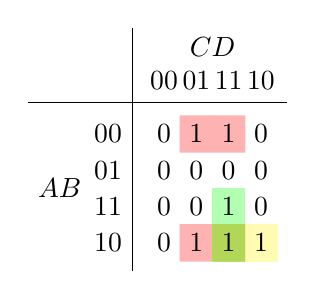
\begin{tikzpicture}
				\matrix (karnaugh) [matrix of math nodes] {
					0 & 1 & 1 & 0 \\
					0 & 0 & 0 & 0 \\
					0 & 0 & 1 & 0 \\
					0 & 1 & 1 & 1 \\
				};

				\foreach \i/\bits in {1/00,2/01,3/11,4/10} {
					\node [left  = 2mm of karnaugh-\i-1] {$\bits$};
					\node [above = 2mm of karnaugh-1-\i] {$\bits$};
				}

				\node [left  = .6cm of karnaugh.west]  (AB) {$AB$};
				\node [above = .5cm of karnaugh.north] (CD) {$CD$};

				\draw	($(CD.north -| karnaugh.west)  + (-.75mm,0)$)
						-- ($(karnaugh.south -| karnaugh.west)  + (-.75mm,0)$)
						($(AB.west |- karnaugh.north) + (0,+.40mm)$)
						-- ($(karnaugh.east |- karnaugh.north) + (0,+.40mm)$);

				\begin{pgfonlayer}{background}
					\begin{scope}[opacity=.3]
						\fill [red]
							(karnaugh-1-2.north west) rectangle (karnaugh-1-3.south east)
							(karnaugh-4-2.north west) rectangle (karnaugh-4-3.south east);
						\fill [yellow]
							(karnaugh-4-3.north west) rectangle (karnaugh-4-4.south east);
						\fill [green]
							(karnaugh-3-3.north west) rectangle (karnaugh-4-3.south east);
					\end{scope}
				\end{pgfonlayer}
			\end{tikzpicture}
		\end{center}
		\caption{
			\label{fig:kmap}
			Karnaugh map of figure \ref{fig:ttable}.
		}
	\end{figure}

	Which shows that equation \ref{eq:booleanexpression} can be represented as the sum of minterms as follows: \begin{equation} f(a,b,c,d)=b'd+acd+ab'c \end{equation}

	% Circuit of gates for k-map'd circuit
	\begin{figure}[h]
		\begin{center}
			\begin{circuitikz} \draw
				(-6.5, 1) node[not port] (not1) {}
				(not1.in) node[left] {$b$}
				(-4, 2) node[and port] (and2) {}
				(not1.out) -| (and2.in 2)
				(and2.in 1) node[left] {$d$}
				(-6, -1) node[and port] (and4) {}
				(and4.in 1) node[left] {$c$}
				(and4.in 2) node[left] {$a$}
				(-4, 0) node[and port] (and3) {}
				(and4.out) -| (and3.in 2)
				(and3.in 1) node[left] {$d$}

				(-2,1) node[or port] (or2) {}
				(and2.out) -| (or2.in 1)
				(and3.out) -| (or2.in 2)

				(-6.5, -3) node[not port] (not2) {}
				(not2.in) node[left] {$b$}
				(-4, -2) node[and port] (and5) {}
				(not2.out) -| (and5.in 2)
				(and5.in 1) node[left] {$a$}
				(-2,-1) node[and port] (and1) {}
				(and1.in 1) node[left] {$c$}
				(and5.out) -| (and1.in 2)

				(0,0) node[or port] (or1) {}
				(or2.out) -| (or1.in 1)
				(and1.out) -| (or1.in 2)
				(or1.out) node[right] {$f_{\sum\text{minterms}}$}
				;
			\end{circuitikz}
		\end{center}
		\caption{
			\label{fig:cdiagram}
			Circuit diagram for equation \ref{eq:booleanexpression} after reduction to sum of midterms.
		}
	\end{figure}

\end{question}

\begin{question}
	Compare the circuits.

	Testing all 16 possible input combinations resulted in identical outputs
	if the gate delay is set to 0ns.
\end{question}

\end{document}
